\documentclass[conference]{IEEEtran}

\usepackage{amsmath}
\usepackage{booktabs}
\usepackage{graphicx}

\title{Cleaning a Simulated Global Temperature Record}

\author{\IEEEauthorblockN{Siva Srinivas Venigalla}}

\begin{document}

\maketitle

\section{Introduction}
The supplied teaching dataset contains simulated monthly global temperature
anomalies from January 1880 through December 2025. I built a reproducible
Python pipeline to repair its deliberately corrupted entries, complete the
monthly record, and calculate normalized values. Fig.~\ref{fig:temperature}
shows the cleaned series with temperature encoded by both position and color.

\section{Data Cleaning}
The pipeline read every field as text, repaired 32 swapped rows, parsed 1,707
data rows, and left no data row unparsed; four trailing non-data lines were
discarded. Sorting and retaining the first record per month removed 20
duplicates. The quartiles were $Q_1=-0.385000$~$^\circ$C and
$Q_3=0.490000$~$^\circ$C, giving an IQR of $0.875000$~$^\circ$C and fences
of $[-1.697500,\,1.802500]$~$^\circ$C. The rule removed 63 outliers, all of
which were $\pm500$ or $\pm999$ sensor codes; it removed no plausible
reading. Reindexing produced all 1,752 months, and linear time interpolation
filled 190 months: 65 absent months and 125 missing values in existing rows.

\section{Normalization}
For each cleaned monthly anomaly $x$, I calculated
\begin{equation}
    d = x - \mu_{20},
    \label{eq:difference}
\end{equation}
and
\begin{equation}
    z = \frac{x - \mu}{\sigma}.
    \label{eq:zscore}
\end{equation}
Here $x$ is the cleaned anomaly in $^\circ$C, $\mu_{20}$ is its mean over
1901--2000, and $d$ is the difference from that baseline used for the color
channel. The symbols $\mu$ and $\sigma$ are the mean and population standard
deviation over 1880--2025, and $z$ is the standardized anomaly. The calculated
values were $\mu_{20}=0.000159$~$^\circ$C, $\mu=0.046434$~$^\circ$C, and
$\sigma=0.519783$~$^\circ$C.

\section{Results}
Calendar-year means used all 12 cleaned monthly values, including interpolated
months. Table~\ref{tab:warmest} lists the five largest annual means.

\begin{table}[!t]
    \caption{Five Warmest Years in the Cleaned Series}
    \label{tab:warmest}
    \centering
    \footnotesize
    \begin{tabular}{@{}rrrr@{}}
        \toprule
        Rank & Year & \shortstack{Mean anomaly\\($^\circ$C)} & Mean $z$ \\
        \midrule
        1 & 2024 & 1.168 & 2.158 \\
        2 & 2023 & 1.153 & 2.130 \\
        3 & 2025 & 1.013 & 1.859 \\
        4 & 2016 & 0.982 & 1.799 \\
        5 & 2022 & 0.960 & 1.759 \\
        \bottomrule
    \end{tabular}
\end{table}

\begin{figure}[!t]
    \centering
    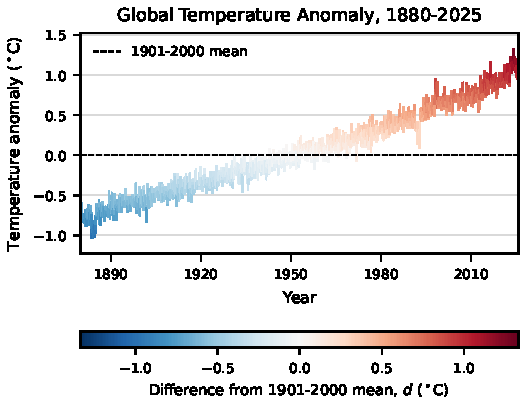
\includegraphics[width=\columnwidth]{temperature_chart.pdf}
    \caption{Cleaned monthly temperature anomaly. Vertical position shows
    $x$, while segment color shows $d$: blue is below and red is above the
    1901--2000 mean. The dashed line marks that baseline.}
    \label{fig:temperature}
\end{figure}

\end{document}
